\documentclass[11pt,class=report,crop=false]{standalone}
\usepackage[screen]{../python}

\begin{document}


%====================================================================
\chapitre{Files}
%====================================================================

\objectifs{You will learn to read and write data with files.}


%%%%%%%%%%%%%%%%%%%%%%%%%%%%%%%%%%%%%%%%%%%%%%%%%%%%%%%%%%%%%%%%
%%%%%%%%%%%%%%%%%%%%%%%%%%%%%%%%%%%%%%%%%%%%%%%%%%%%%%%%%%%%%%%%
\begin{cours}[Write to a file]

\index{file}

Writing to a file is almost as easy as displaying a sentence on the screen.
On the left is a program that writes two lines to a file called \ci{my_file.txt}; on the right is the resulting file that is displayed in a text editor.
\begin{center}
\begin{minipage}{0.5\textwidth}
\begin{lstlisting}
fi = open("my_file.txt","w")

fi.write("Hello world!\n")

line = "Hi there.\n"
fi.write(line)

fi.close()
\end{lstlisting}
\end{minipage}
\begin{minipage}{0.3\textwidth}
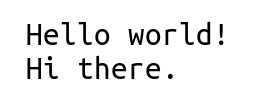
\includegraphics[scale=\myscale,scale=0.5]{screen-files-lesson-1-en}
\end{minipage}
\end{center}


\textbf{Explanations.}
\begin{itemize}
  \item The command \ci{open}\index{open@\ci{open}} allows you to open a file. The first argument is the name of the file. The second argument here is \ci{"w"} to say that you want to write to the file.
  
  \item We do not work with the file name, but with the value returned by the function \ci{open}. Here we have named this object file \ci{fi}. From now on we will work with this variable \ci{fi}.
  
  \item We now write in the file almost as we would display a sentence on the screen. The instruction is \ci{fi.write()}\index{write@\ci{write}} where the argument is a string of characters.
  
  \item To switch to the next line, you must add the line terminator character \ci{"\\n"}.
  
  \item It is important to close your file when you are finished writing. The instruction is \ci{fi.close()}.\index{close@\ci{close}} 
   
  \item The data to be written is composed of strings, so to write a number, you must first transform it using \ci{str(number)}.\index{str@\ci{str}}
\end{itemize}
  
  
\end{cours}


\begin{cours}[Read a file]

It is just as easy to read a file.
Here is how to do it (left) and the display by \Python{} on the screen (right).
\begin{center}
\begin{minipage}{0.5\textwidth}
\begin{lstlisting}
fi = open("my_file.txt","r")

for line in fi:
    print(line)

fi.close()
\end{lstlisting}
\end{minipage}
\begin{minipage}{0.3\textwidth}
\begin{lstlisting}
Hello world!

Hi there.
\end{lstlisting}
\end{minipage}
\end{center}

\textbf{Explanations.}
\begin{itemize}
  \item The command \ci{open} is called with the argument \ci{"r"} (for read) this time, it opens the file in reading.
  
  \item We work again with an object file here named \ci{fi}.
  
  \item A loop goes through the entire file line by line. Here we just ask to display each line.
  
  \item We close the file with \ci{fi.close()}.  
  
  \item The data read is a string, so if you want a number, you must first transform it with \ci{int(string)}\index{int@\ci{int}} (for an integer) or  
  \ci{float(string)}\index{float@\ci{float}} (for a decimal number).

\end{itemize}
  
\end{cours}



%%%%%%%%%%%%%%%%%%%%%%%%%%%%%%%%%%%%%%%%%%%%%%%%%%%%%%%%%%%%%%%%
% Activity 1
%%%%%%%%%%%%%%%%%%%%%%%%%%%%%%%%%%%%%%%%%%%%%%%%%%%%%%%%%%%%%%%%

\begin{activite}[Read and write a file]

\objectifs{Goal: write a file of grades, then read it to calculate the averages.}

\begin{enumerate}
  \item Generate at random a grades file, named \ci{grades.txt}, which is composed of lines with the structure: 
  \mycenterline{\ci{Firstname Lastname grade1 grade2 grade3}} 
  
  For example:
\begin{center}
\begin{minipage}{0.5\textwidth}
\begin{lstlisting}
Tintin Vador 15.0 5.0 19.0
Bill Croft 15.0 14.5 10.5
Hermione Skywalker 10.5 7.0 19.5
Lara Parker 12.5 13.0 14.5
Hermione Croft 11.5 18.5 9.5
Robin Vador 8.0 8.0 11.0
\end{lstlisting}
\end{minipage}
\end{center}  
  
%\begin{center}
%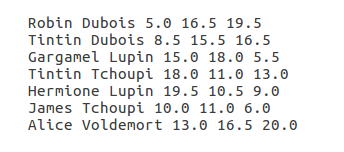
\includegraphics[scale=\myscale,scale=0.7]{screen-files-1a}
%\end{center} 

  \emph{Hints.}
  \begin{itemize}
    	\item Build a list of first names \ci{list_firstnames = ["Alice","Tintin","James",...]}. Then choose a first name at random by the instruction \ci{firstname = choice(list_firstnames)}\index{choice@\ci{choice}} (you have to import the module \ci{random}).
    	
    	\item Do the same thing for last names! 
    	
    	\item For a grade, you can choose a random number with the command \ci{randint(a,b)}. 
    	
    	\item \textbf{Please note!} Don't forget to convert the numbers into a string to write it to the file: \ci{str(grade)}.
    	
   \end{itemize}
    
  
  \item Read the file \ci{grades.txt} that you produced. Calculate the average of each person's grades and write the result to a file \ci{averages.txt} where each line is of the form:   
  \mycenterline{\ci{Firstname Lastname average}} 
 
For example:  
\begin{center}
\begin{minipage}{0.5\textwidth}
\begin{lstlisting}
Tintin Vador 13.00
Bill Croft 13.33
Hermione Skywalker 12.33
Lara Parker 13.33
Hermione Croft 13.17
Robin Vador 9.00
\end{lstlisting}
\end{minipage}
\end{center}   
  

%    
%\begin{center}
%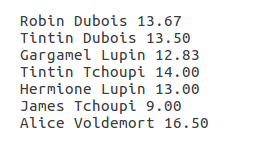
\includegraphics[scale=\myscale,scale=0.7]{screen-files-1b}
%\end{center}  

  \emph{Hints.}
  \begin{itemize}
    	\item For each line read from the file \ci{grades.txt}, you get the data as a list by using the command \ci{line.split()}.
    	
    	\item \textbf{Please note!} The data read is a string. You can convert a string \ci{"12.5"} to the number \ci{12.5} by using the instruction \ci{float(string)}.
    	
    	\item To convert a number to a string with only two decimal places after the dot, you can use the command \ci{'\{0:.2f\}'.format(number)}.
    	
    	\item Don't forget to close all your files.
    	
   \end{itemize}
    
\end{enumerate}   
     
\end{activite}


%%%%%%%%%%%%%%%%%%%%%%%%%%%%%%%%%%%%%%%%%%%%%%%%%%%%%%%%%%%%%%%%
%%%%%%%%%%%%%%%%%%%%%%%%%%%%%%%%%%%%%%%%%%%%%%%%%%%%%%%%%%%%%%%%

\begin{cours}[Files with format \emph{csv}]
The format \emph{csv}\index{csv@\emph{csv}} (for \emph{comma-separated values}) is a very simple text file format containing data.
Each line of the file contains a series of values (numbers or text). On the same line the values are separated by a comma (hence the name of the format, even if other separators are possible).

\medskip

\textbf{Example.} Here is a file that contains the names, first names, years of birth, height and number of Nobel Prize medals:
\begin{center}
\begin{minipage}{0.4\textwidth}
\begin{lstlisting}
CURIE,Marie,1867,1.55,2
EINSTEIN,Albert,1879,1.75,1
NOBEL,Alfred,1833,1.70,0
\end{lstlisting}
\end{minipage}
\end{center}

\end{cours}

%\medskip

%%%%%%%%%%%%%%%%%%%%%%%%%%%%%%%%%%%%%%%%%%%%%%%%%%%%%%%%%%%%%%%%
% Activity 2
%%%%%%%%%%%%%%%%%%%%%%%%%%%%%%%%%%%%%%%%%%%%%%%%%%%%%%%%%%%%%%%%


\begin{activite}[csv format]

\objectifs{Goal: write a data file, with the \emph{csv} format, then read it for a graphic display.}

\begin{enumerate}
  \item Generate a \ci{sales.csv} file of sales figures (randomly drawn) from a sports brand.
  
Here is an example:
\begin{center}
\begin{minipage}{0.4\textwidth}
\begin{lstlisting}
Best sales of the brand 'Pentathlon'

,2015,2016,2017,2018,2019,2020

Mountain bike,560,890,500,550,650,970
Surfboard,550,690,750,640,710,790
Running shoes,850,740,790,1000,680,540
Badminton racket,710,640,620,550,790,880
Volley ball,900,550,790,510,930,800
\end{lstlisting}
\end{minipage}
\end{center}
%\begin{center}
%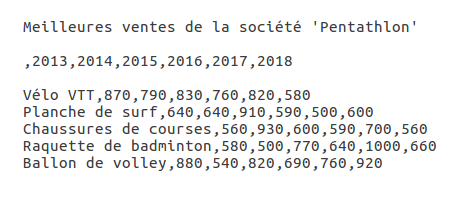
\includegraphics[scale=\myscale,scale=0.6]{screen-files-2a}
%\end{center} 

\begin{itemize}
  \item The data starts from the fifth line.
  \item The produced file respects the format \emph{csv} and can be readable by
   \emph{LibreOffice Calc} for example.
\end{itemize}

\begin{center}
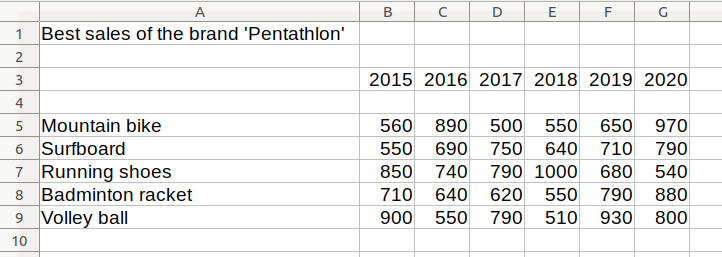
\includegraphics[scale=\myscale,scale=0.45]{screen-files-2b-en}
\end{center} 

  \item Read the file \ci{sales.csv} to display the sales curves.
  \begin{center}
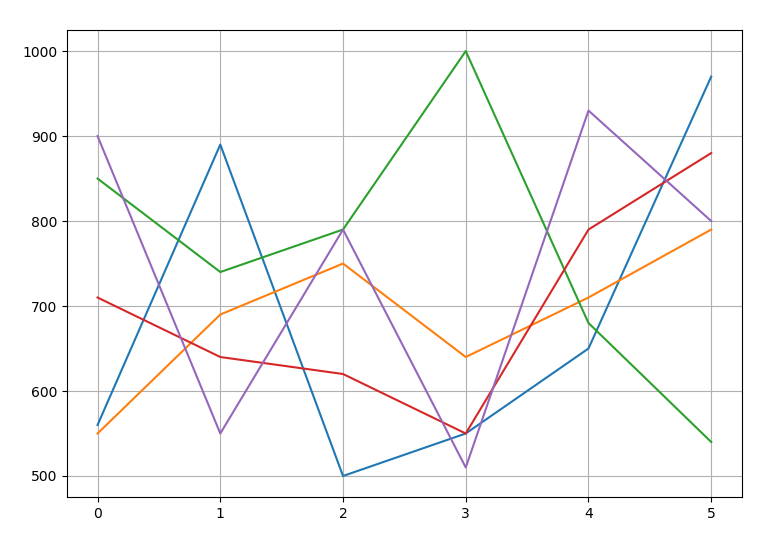
\includegraphics[scale=\myscale,scale=0.4]{screen-files-2c-en}
\end{center}  

  \emph{Hints.} 
  \begin{itemize}
    	\item The \ci{matplotlib} package allows you to easily display graphics, it is often called with the instruction:  	
   \mycenterline{\ci{import matplotlib.pyplot as plt}}  
   
   \item Here is how to view two data lists \ci{mylist1} and \ci{mylist2}:
\begin{center}
\begin{minipage}{0.4\textwidth}
\begin{lstlisting}
plt.plot(mylist1)
plt.plot(mylist2)
plt.grid()
plt.show()
\end{lstlisting}
\end{minipage}
\end{center}


   \end{itemize}
\end{enumerate}   
     
\end{activite}

%%%%%%%%%%%%%%%%%%%%%%%%%%%%%%%%%%%%%%%%%%%%%%%%%%%%%%%%%%%%%%%%
%%%%%%%%%%%%%%%%%%%%%%%%%%%%%%%%%%%%%%%%%%%%%%%%%%%%%%%%%%%%%%%%


\begin{cours}[Images \emph{bitmap}]

\index{pbm@\emph{pbm/pgm/ppm}}
\index{image}

There is a simple file format, called the \emph{bitmap} format, which describes an image pixel by pixel. This format is available in three variants 
depending on whether the image is in black and white, grayscale, or color.

\medskip

\textbf{Black and white picture, format \og{}pbm\fg{}.}

The image is described by $1$'s and $0$'s.

Here is an example: the file \ci{image_bw.pbm} is on the left (read as a text file) and on the right is its visualization (using an image reader, here very enlarged).
\begin{center}
\begin{minipage}{0.3\textwidth}
\begin{lstlisting}
P1
4 5
1 1 1 1
1 0 0 0
1 1 1 0
1 0 0 0
1 1 1 1
\end{lstlisting}
\end{minipage}
\begin{minipage}{0.3\textwidth}

\includegraphics[scale=\myscale,scale=0.2]{screen-lesson-image_nb}
\end{minipage}
\end{center}

Here is the description of the format:
\begin{itemize}
  \item First line: the id \ci{P1}.
  \item Second line: the number of columns, then the number of rows (here 4 columns and 5 rows).
  \item Then the color of each pixel line by line: \ci{1} for a black pixel, \ci{0} for a white pixel. Warning: this is contrary to the usual convention!
\end{itemize}  
  
\medskip

\textbf{Grayscale image, format \og{}pgm\fg{}.}

The image is described by different values for different grayscales.
Here is an example: the file \ci{image_gray.pbm} is on the left and on the right is its visualization.
\begin{center}
\begin{minipage}{0.3\textwidth}
\begin{lstlisting}
P2
4 5
255
  0   0   0   0
192 192 192 192
192 255 128 128
192 255  64  64
192   0   0   0
\end{lstlisting}
\end{minipage}
\begin{minipage}{0.3\textwidth}

\includegraphics[scale=\myscale,scale=0.2]{screen-lesson-image_gris}
\end{minipage}
\end{center}

Here is the description of the format:
\begin{itemize}
  \item First line: the identifier is this time \ci{P2}.
  \item Second line: the number of columns, then the number of rows.
  \item Third line: the maximum value of the grayscale (here $255$).
  \item Then the grayscale of each pixel line by line: this time \ci{0} for a black pixel, the maximum value for a white pixel and intermediate values give intermediate grays. 
\end{itemize}  

\medskip

\textbf{Image in colors, format \og{}ppm\fg{}.}


The image is described by three values per pixel: one for red, one for green, and one for blue.

Here is an example: the file \ci{image_col.ppm} on the left and on the right its visualization.
\begin{center}
\begin{minipage}{0.6\textwidth}
\begin{lstlisting}
P3
3 2
255
255   0   0     0 255 0     0   0 255
  0 128 255   255 128 0   128 255   0
\end{lstlisting}
\end{minipage}
\begin{minipage}{0.3\textwidth}
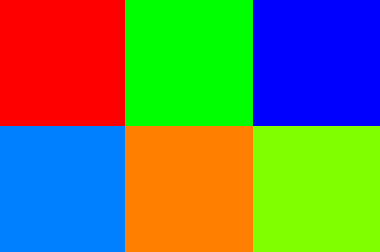
\includegraphics[scale=\myscale,scale=0.2]{screen-lesson-image_coul}
\end{minipage}
\end{center}

Here is the description of the format:
\begin{itemize}
  \item First line: the id is now \ci{P3}.
  \item Second line: the number of columns, then the number of rows.
  \item Third line: the maximum value of the color levels (here $255$).
  \item Then each pixel is described by $3$ numbers: the level of red, green and blue (RGB system)\index{rgb@\emph{rgb}}. For example, the first pixel is encoded by $(255,0,0)$ so it is a red pixel.
\end{itemize} 


\end{cours}


%%%%%%%%%%%%%%%%%%%%%%%%%%%%%%%%%%%%%%%%%%%%%%%%%%%%%%%%%%%%%%%%
% Activity 3
%%%%%%%%%%%%%%%%%%%%%%%%%%%%%%%%%%%%%%%%%%%%%%%%%%%%%%%%%%%%%%%%

\begin{activite}[Images \emph{bitmap}]

\objectifs{Goal: define your own images pixel by pixel.}


\begin{enumerate}
  \item Generate a file \ci{image_bw.pbm} that represents a black and white image (e.g. of size $300 \times 200$) according to the following pattern:
\begin{center}

\includegraphics[scale=\myscale,scale=0.5]{screen-image_nb}
\end{center}   

\emph{Hints.} If $i$ designates the line number and $j$ the column number (from the top left), then the pixel in position $(i,j)$ is white if $i+j$ is between $0$ and $9$, between $20$ and $29$, or between $40$ and $49$,\ldots{} This is obtained by the formula :
\mycenterline{\ci{col = (i+j)//10 \% 2}}
which returns $0$ or $1$ as desired.

  \item Generate a file \ci{image_gray.pgm} that represents a grayscale image (for example of size $200 \times 200$ with $256$ grayscale) according to the following pattern:
\begin{center}
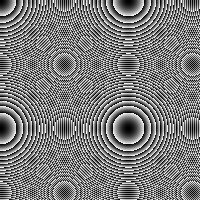
\includegraphics[scale=\myscale,scale=0.7]{screen-image_gris}
\end{center}   

\emph{Hints.} This time the formula is:
\mycenterline{\ci{col = (i**2 + j**2) \% 256}}
which returns an integer between $0$ and $255$.

   \item Generate a file \ci{image_col.ppm} that represents a color image (e.g. of size $200 \times 200$, with $256$ red, green and blue levels) according to the following pattern:
\begin{center}
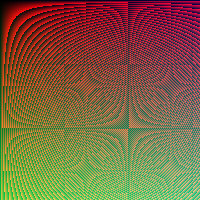
\includegraphics[scale=\myscale,scale=0.7]{screen-image_coul}
\end{center}   

\emph{Hints.} This time the formulas are:
\mycenterline{\ci{R = (i*j) \% 256}}
\mycenterline{\ci{G = i \% 256}}
\mycenterline{\ci{B = (i + j)//3 \% 256}}
which gives the red, green and blue levels of the pixel $(i,j)$.

\item Write a function \ci{inverse_black_white(filename)} that reads a black and white image file \ci{.pbm} and creates a new file in which the white pixels have turned black and vice versa. 

Example: on the left the start image, on the right the finish image.
\begin{center}

\includegraphics[scale=\myscale,scale=0.3]{screen-simple_nb}\qquad\qquad

\includegraphics[scale=\myscale,scale=0.3]{screen-simple_nb_inverse}
\end{center} 

\item Write a function \ci{colors_to_gray(filename)} that reads a color image file in \ci{.ppm} format and creates a new file in \ci{.pgm} format in which the color pixels are transformed into grayscale. 

You can use the formula: \index{rgb@\emph{rgb}}
$$g = 0,21 \times R \  + \  0,72 \times G \  + \  0,07 \times B$$
where
\begin{itemize}
  \item $R,G,B$ are the red, green and blue levels of the colored pixel,
  \item $g$ is the grayscale of the transformed pixel.
\end{itemize}

Example: on the left the starting image in color, on the right the arrival image in grayscale.
\begin{center}
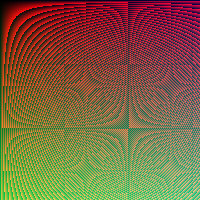
\includegraphics[scale=\myscale,scale=0.5]{screen-image_coul}\qquad\qquad
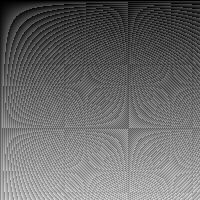
\includegraphics[scale=\myscale,scale=0.5]{screen-image_coul_gris}
\end{center} 


\end{enumerate}   
     
\end{activite}


%%%%%%%%%%%%%%%%%%%%%%%%%%%%%%%%%%%%%%%%%%%%%%%%%%%%%%%%%%%%%%%%
% Activity 4
%%%%%%%%%%%%%%%%%%%%%%%%%%%%%%%%%%%%%%%%%%%%%%%%%%%%%%%%%%%%%%%%


\begin{activite}[Distance between two cities]

\objectifs{Goal: read the coordinates of the cities and write the distances between them.}
\index{distance}

\begin{enumerate}
  \item \textbf{Distance in the plan.} 
  
  Write a program that reads a file containing the coordinates $(x,y)$ of cities, then calculates and writes in another file the distances (on the map) between two cities.
  
  The formula for the distance between two points $(x_1,y_1)$ and $(x_2,y_2)$ of the plane is:
  $$d = \sqrt{(x_2-x_1)^2 + (y_2-y_1)^2}.$$
  
  
\textbf{Example.} Here is an example of an input file:
\begin{center}
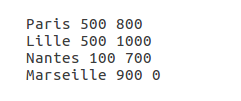
\includegraphics[scale=\myscale,scale=0.7]{screen-files-4a}
\end{center}   

And here is the output file produced by the program:
\begin{center}
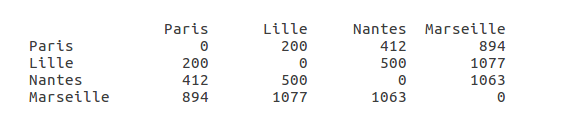
\includegraphics[scale=\myscale,scale=0.7]{screen-files-4b} 
\end{center}   
We can read from this file that the distance between Lille and Marseille is $1077$ kilometers.


Below is the map of France that provides (very approximate) data for the input file. The origin is at the bottom left, each side of a square represents $100$ km. For example, in this diagram, Paris has the coordinates $(500,800)$.
 
 \myfigure{0.6}{
  \tikzinput{fig-france}
} 

  \item \textbf{Distance on the sphere.} 
  
On Earth, the distance between two cities is a distance on a \emph{great circle} along the surface of the sphere and not along a straight line. This is the distance a plane travels to connect two cities.

 Write a program that reads the latitudes and longitudes of cities, then calculates and writes to another file the distances (on the Earth's surface) between two cities. 
  
\textbf{Example.} Here is an example of an input file:
\begin{center}
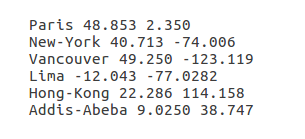
\includegraphics[scale=\myscale,scale=0.7]{screen-files-4c}
\end{center}   

And here is the output file produced by the program:
\begin{center}
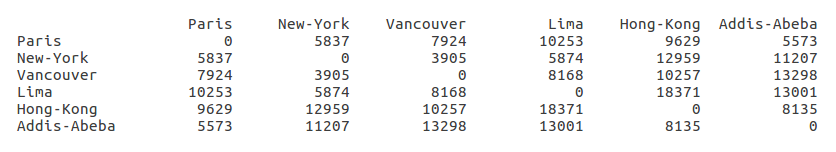
\includegraphics[scale=\myscale,scale=0.55]{screen-files-4d} 
\end{center}  
    
    
\textbf{Implementation and explanations.}

\begin{itemize}
	\item The input file contains the latitude (noted as $\varphi$) and longitude (noted as $\lambda$) in degrees for each city. For example, Paris has a latitude of $\varphi = 48.853$ degrees and a longitude of $\lambda = 2.350$ degrees.
	
	\item It will be necessary to use the angles in radians for the formulas. The formula for converting degrees to radians is: \index{angle}\index{degrees}\index{radians}
	$$\text{angle in radians} = \frac{2\pi}{360} \times \text{angle in degrees}$$
		
	\item \textbf{Formula for an approximate distance.}
	
	There is a simple formula that gives a good estimate for the shortest distance between two points on a sphere with a radius of $R$.
    First, let:
    $$x =   (\lambda_2-\lambda_1)\cdot  \cos\left( \frac{\varphi_1+\varphi_2}{2} \right)
    \quad\text{ and }\quad 
    y = \varphi_2-\varphi_1$$
	The approximate distance is then 
	$$ \tilde d = R \sqrt{x^2 + y^2}$$		
	where $(\varphi_1,\lambda_1)$ and $(\varphi_2,\lambda_2)$ are the latitudes/longitudes of two cities expressed in radians.
	
	\item \textbf{Exact distance formula.}
	
	The bravest can use the exact formula to calculate the distance.
	First, set: 
	$$a = \left(\sin\left(\frac{\varphi_1+\varphi_2}{2}\right)\right)^2 + \cos(\varphi_1)\cdot \cos(\varphi_2) \cdot \left(\sin\left( \frac{\lambda_2-\lambda_1}{2} \right)\right)^2$$
    The exact distance is then:
    $$d = 2 \cdot R \cdot \text{atan2}\left(\sqrt{a},\sqrt{1-a}\right)$$
    where $\text{atan2}(y,x)$ is the function \og{}arctangent\fg{} which is obtained by the command \ci{atan2(y,x)} from the module \ci{math}.	
	
	\item For the Earth radius we will take $R = 6371$ km.

\end{itemize}
  
\end{enumerate}   
     
\end{activite}


\end{document}
